%Η επαναφορά της ηλεκτρασθενούς συμμετρίας είναι συνέπεια της %αναίρεσης του εκφυλισμού της κατάστασης κενού. 
Ο εκφυλισμός του κενού της ηλεκτρασθενούς θεωρίας αίρεται στην παρουσία ισχυρών μαγνητικών πεδίων, τα οποία θέτουν την αναμενόμενη τιμή του βαθμωτού πεδίου Higgs ίση με μηδέν: $\left<\phi\right>\rightarrow0$. Η μηδενική τιμή είναι  αναλλοίωτη ως προς τη δράση της ομάδας της ηλεκτρασθενούς συμμετρίας \eqref{vacuum exp value symmetry group action}, και η αντίστοιχη κατάσταση κενού είναι συμμετρική. 

\section{Κορώνα Ηλεκτρασθενούς συμμετρίας}
%Οι μελανές οπές συνιστούν φυσικές διαμορφώσεις που μπορούν να %υποστηρίξουν μαγνητικά πεδία μονοπολικής μορφής και ισχύος %ικανής να διαταράξει το συνηθισμένο ηλεκτρομαγνητικό κενό.
Η ένταση του μαγνητικού πεδίου μιας ακραίας, μαγνητικά φορτισμένης μαύρης τρύπας μεταβάλλεται με την απόσταση σύμφωνα με τον κανόνα του αντιστρόφου τετραγώνου
\begin{equation}
    |F|\equiv eB = \frac{Q}{2r\superscr{2}}
\end{equation}
Η ένταση αυτή έχει μονάδες $(eV)\superscr{2}$. Η μέγιστη τιμή επιτυγχάνεται στον ορίζοντα $r\subscr{e}=\frac{Q\sqrt{\pi G}}{e}$ και δίδεται από την έκφραση
\begin{equation}
    |F|=\frac{e\superscr{2}}{2\pi G\superscr{2}Q}
\end{equation}
Παρατηρούμε ότι η μέγιστη αυτή τιμή ελαττώνεται όταν αυξάνεται το μαγνηικό φορτίο $Q$.\\

Διάφορα φαινόμενα που οδηγούν τελικά στην αποκατάσταση της ηλεκτρασθενούς συμμετρίας λαμβάνουν χώρα, όταν το μαγνητικό φορτίο είναι μικρότερο από μια οριακή τιμή $Q\subscr{ew}$, που καθορίζεται από την ενεργειακή κλίμακα στην οποία σπάζει η συμμετρία. 
%Για σχετικά μικρό φορτίο 
Εάν $Q<Q\subscr{ew}$, υπάρχουν δύο κρίσιμες ακτίνες, $r\subscr{h}$ και $r\subscr{w}$, στις οποίες η ένταση του μαγνητικού πεδίου παίρνει τιμές ίσες με τα τετράγωνα των μαζών του πεδίου Higgs και των μποζονίων $W$, $m\subscr{h}\superscr{2}\equiv 4\lambda v\superscr{2}$ και $m\subscr{w}\superscr{2}\equiv \frac{g\superscr{2}v\superscr{2}}{2}$, αντίστοιχα:
\begin{equation}
    r\subscr{h}=\sqrt{\frac{Q}{2}}\frac{1}{m\subscr{h}}\quad < \quad r\subscr{w}=\sqrt{\frac{Q}{2}}\frac{1}{m\subscr{w}}
\end{equation}
Όταν το μαγνητικό φορτίο ισούται με την οριακή τιμή $Q\subscr{ew}$, η ακτίνα του ορίζοντα $r\subscr{e}$ ισούται με την ακτίνα $r\subscr{w}$
\begin{equation}
    r\subscr{e}(Q\subscr{ew})=r\subscr{w}(Q\subscr{ew})\qquad Q\subscr{ew}=\frac{e\superscr{2}}{2\pi G m\superscr{2}\subscr{w}}
\end{equation}
Στην περίπτωση αυτή δεν μπορεί να σχηματιστεί η ηλεκτρασθενής κορώνα και τα φαινόμενα δεν λαμβάνουν χώρα.\\ 

Σε ακτίνες $r\le r\subscr{w}$, η κατάσταση κενού (με σπασμένη την ηλεκτρασθενή συμμετρία) δεν είναι ευσταθής επειδή τα μποζόνια $W$ γίνονται ταχυονικά. Δημιουργούνται συμπυκνώματα μποζονίων $W$ και το σύστημα μεταβαίνει σε μια νέα κατάσταση κενού με χαμηλότερη ενέργεια. Καθώς η ακτίνα ελαττώνεται, η αναμενόμενη τιμή του πεδίου Higgs ελαττώνεται από την αρχικά μη μηδενική της τιμή στη μηδενική τιμή όταν $r=r_h$. Για ακτίνες $r_e<r<r_h$ η αναμενόμενη τιμή του Higgs είναι μηδενική και έτσι έχουμε επαναφορά της ηλεκτρασθενούς συμμετρίας. 
%μεταβολή του κενού ισοδυναμεί με την μη ευστάθεια του ίδιου του %πεδίου το οποίο υποκύπτει στην καινούρια, ευσταθή μορφή. Η %μετάβαση από το μοντέλο με τη κατάσταση κενού %$\left<\phi\right>\ne0$ που σπάζει τη συμμετρία, στο μοντέλο με %τη συμμετρική κατάσταση κενού, $\left<\phi\right>=0$ είναι %συνεχής και γίνεται εντός του διαστήματος $r\subscr{h}\le r\le %r\subscr{w}$. 
Η ενδιάμεση περιοχή $r\subscr{h}\le r\le r\subscr{w}$ είναι η ηλεκτρασθενής κορώνα. Το συμπύκνωμα μποζονίων $W$ θωρακίζε το μαγνητικό πεδίο $SU(2)$. Μάλιστα, όταν $|F|>m\superscr{2}\subscr{h}$ (ισοδύναμα $r<r\subscr{h}$) στο μαγνητικό πεδίο συνεισφέρει μόνο η $U(1)$ συνιστώσα του υπερφορτίου. 
%πλέον μόνο με την αβελιανή ομάδα υπερφορτίου %$U(1)\subscr{\text{y}}$. Η SU(2) συνιστώσα του πεδίου %θωρακίζεται.

\section{Μετάβαση στην περιοχή ηλεκτρασθενούς συμμετρίας}
%Στην QED θεωρεία, η παρουσία μόνο των spin-½ Dirac σωματιδίων %επιτρέπει την ευστάθεια της κατάστασης κενού εντός ισχυρών %μαγνητικών πεδίων - οι συνεισφορές στροφορμής και σύζευξης spin %με μαγνητικό πεδίο αλληλοαναιρούνται για το κατώτατο επίπεδο %Landau, και έτσι η ενέργεια \eqref{spinor energy magnetic %field} είναι ανεξάρτητη της μαγνητικής έντασης |F|. Σε ανώτερα %επίπεδα Landau n, η συνεισφορά του μαγνητικού πεδίου %εξακολουθεί να είναι ασφαλής από αστάθειες %($E\superscr{2}\subscr{n}>0$). 
Στην ηλεκτρασθενή θεωρία 
%όμως, οι κβαντικές διακυμάνσεις του κενού περιέχουν τα %μποζονικά πεδία των ασθενών αλληλεπιδράσεων, των οποίων 
η σύζευξη των φορτισμένων μποζονικών πεδίων $W$ με το μαγνητικό πεδίο 
%φένεται να 
οδηγεί σε αστάθειες. Στην παρουσία μαγνητικού πεδίου, η ενεργός μάζα στο τετράγωνο των μποζονίων $W$ (τα οποία έχουν σπιν 1 και μη μηδενικό ηλεκτρικό φορτίο) είναι \cite{AMBJORN1990193,ambjornTheoryAndApplications} 
%των Ambjorn και Olesen, παρουσιάζεται ότι, στη σπασμένη %ηλεκτρασθενή θεωρία, και για τιμές της έντασης 
%, η %ενέργεια  των spin-1 μποζονίων
\begin{equation}
    m\superscr{2}_{eff}= -(|F|-m\subscr{W}\superscr{2})
\end{equation}
εξαιτίας της σύζευξης του σπιν με το μαγνητικό πεδίο.
Επομένως, όταν η ένταση του μαγνητικού πεδίου είναι αρκετά μεγάλη, $|F|> m\subscr{W}\superscr{2}\sim \text{10}\superscr{20}\,T$, 
η ενεργός μάζα στο τετράγωνο γίνεται αρνητική
%αποκτά μιγαδικό χαραχτήρα (και κατά συνέπεια η ενέργεια της %κατάστασης κενού), λόγω του αρνητικού προσίμου στην %\eqref{vector boson energy magnetic field} που προήλθε από τη . %Ως αποτέλεσμα, η θεωρία υποφέρει από ανωμαλίες καθώς 
και τα μποζόνια $W$ ταχυονικά. Η ύπαρξη ταχυονικών σωματιδίων στο φάσμα υποδηλώνει ότι η κατάσταση κενού είναι ασταθής, με αποτέλεσμα τη δημιουργία συμπυκνωμάτων μποζονίων $W$ και τη μετάβαση σε μια νέα ευσταθή κατάσταση κενού.\\
%Οι Ambjorn και Olesen ανατρέχουν πίσω στην πλήρη ηλεκτρασθενή %θεωρία, και διορθώνουν τις ανωμαλίες συνδυάζοντας τα ισχυρά %μαγνητικά πεδία με συμπύκνωμα (condensate) των μποζονίων W. 

Άρα λοιπόν, στην παρουσία ισχυρών μαγνητικών πεδίων, $|F|\equiv eF\subscr{12}\ge m\subscr{w}\superscr{2}$, η αρχική κατάσταση κενού, 
%(παρουσία ισχυρών ηλεκτρομαγνητικών πεδίων) δεν είναι η %συμβατική
η οποία χαρακτηρίζεται από σπάσιμο της ηλεκτρασθενούς συμμετρίας και τις ακόλουθες αναμενόμενες τιμές για τους πεδιακούς τελεστές ${\scriptstyle\left<\phi\right>\,>\,}0$, ${\scriptstyle\left<W\subscr{\mu}\right>\,=\,\left<Z\subscr{\mu}\right>\,=\,}0$ δεν είναι ευσταθής. Θα πρέπει να προσδιορίσουμε τις καταστάσεις που ελαχιστοποιούν την ενέργεια. 
%Η διερεύνηση πραγματοποιείται 
Θα εργαστούμε στη βαθμίδα όπου το πεδίο Higgs 
%είναι η πραγματική SU(2) διπλέτα
έχει τη μορφή
\begin{equation}
    \left(\begin{array}{c}0 \\ \phi\end{array}\right)
\end{equation}
με τη μη μηδενική συνιστώσα να είναι πραγματική. Η αναμενώμενη τιμή της συνιστώσας αυτής θα προσδιοριστεί συναρτήσει του συμπυκνώματος $W$.
%αλλά δεν λαμβάνει την συνήθη αναμενόμενη τιμή \eqref{real %scalar doublet}, και αφήνεται να προσδιοριστεί κατά την %ελαχιστοποίηση, συναρτήσει του συμπηκνώματος W. 
Οι μόνες μη μηδενικές συνιστώσες των αναλλοίωτων τανυστών 
%των φυσικών πεδίων θεωρούνται με μόνο τα στοιχεία %$F\subscr{12}$ και $Z\subscr{12}$ μη μηδενικά και επίσης θα %προσδιοριστούν από τις απορρέουσες εξισώσεις. Ισχύουν οι %ορισμοί
\begin{subequations}
    \begin{equation}
        F\subscr{\mu\nu}=\partial\subscr{\mu}A\subscr{\nu}-\partial\subscr{\nu}A\subscr{\mu}
    \end{equation}
    \begin{equation}
        Z\subscr{\mu\nu}=\partial\subscr{\mu}Z\subscr{\nu}-\partial\subscr{\nu}Z\subscr{\mu}
    \end{equation}
\end{subequations}
είναι οι μαγνητικές $F\subscr{12}=-F\subscr{21}$ και $Z\subscr{12}=-Z\subscr{21}$, οι οποίες θα προσδιοριστούν από τις εξισώσεις της θεωρίας.
%Το ηλεκτρομαγνητικό δυναμικό καθορίζεται 
Εργαζόμαστε στη βαθμίδα Landau με το ηλεκτρομαγνητικό δυναμικό να δίδεται από την έκφραση 
%(αντιστοιχεί στο συμβατικό αβελιανό μαγνητικό πεδίο)
\begin{equation}
    A\subscr{\mu}=x\subscr{1}\frac{|F|}{e}\de\subscr{\mu 2}
\end{equation}
Το υπόβαθρο μαγντικό πεδίο θεωρείται ομογενές, και εργαζόμαστε στο κάθετο επίπεδο. Η γενίκευση για σφαιρική επιφάνεια κάθετη σε μονοπολικό πεδίο 
%(όπως αρμόζει στο θέμα της διατριβής) 
είναι άμεση.\\ 

Η λαγκραντζιανή του ηλεκτρασθενούς μοντέλου δίνεται στην εξίσωση \eqref{electroweak lagragian in terms of physical fields}. Η πυκνότητα ενέργειας αποτελεί άθροισμα τέλειων τετραγώνων \cite{AMBJORN1990193,ambjornTheoryAndApplications} 
%ως άθροισμα τετραγωνικών όρων 
και συνεπώς ο κάθε όρος πρέπει να μηδενίζεται για την ελαχιστοποίηση ελαχιστοποίηση της. Όταν οι σταθερές σύζευξης $\lambda$ (στο δυναμικό Higgs) και $g$ (της $SU(2)\subscr{L}$ ομάδας) συνδέονται με τη σχέση
\begin{equation}
    \lambda=\frac{g\superscr{2}}{8\cos\superscr{2}\theta\subscr{w}}
\end{equation}
η ελαχιστοποίηση της ενέργειας επιτυγχάνεται όταν 
%"αναγκάζει" τις 
οι κάθετες στο μαγνητικό πεδίο συνιστώσες του δυναμικού $W\subscr{\mu}$ είναι μη μηδενικές και παίρνουν τη μορφή 
%να αποκτίσουν μη μηδενική αναμενόμενη τιμή και περιορίζονται %από το ακόλουθο anzats
\begin{equation}\label{ansatz for W field}
    W\subscr{0}=W\subscr{3}=0,\quad W\subscr{1}=-iW\subscr{2}=W(x\subscr{1}+ix\subscr{2}),\qquad W \in \mathbb{C}
\end{equation}
%όπου 1 και 2 είναι οι κάθετες διευθύνσεις στο μαγνητικό πεδίο. 
Με βάση την \eqref{ansatz for W field}, οι σχετικές πεδιακές εξισώσεις ανάγονται στις ακόλουθες \cite{AMBJORN1990193,ambjornTheoryAndApplications} 
\begin{english}
\begin{subequations}
  \begin{equation}
    \label{de for W condensation function}
        (D\subscr{1}+iD\subscr{2})W=0,\qquad D\subscr{i}\equiv\partial\subscr{i}-ig(\sin\theta\subscr{w} A\subscr{i}+\cos\theta\subscr{w} Z\subscr{i})
    \end{equation}
  \begin{equation}
    \label{equation for f12}
        F\subscr{12}=\frac{g}{2\sin\theta\subscr{w}}v\superscr{2}+2g\sin\theta\subscr{w}|W|\superscr{2}
  \end{equation}
  \begin{equation}
    \label{equation for Z12}
        Z\subscr{12}=\frac{g}{2\cos\theta\subscr{w}}(\phi\superscr{2}-v\superscr{2})+2g\cos\theta\subscr{w}|W|\superscr{2}
  \end{equation}
  \begin{equation}
    \label{equation for Zi}
        Z\subscr{i}=-\frac{2\cos\theta\subscr{w}}{g}\epsilon\subscr{ij}\partial\subscr{j}\ln\phi\qquad i=1,2
  \end{equation}
\end{subequations}
\end{english}
όπου $v\equiv\,{\scriptstyle\left|\left<\phi\subscr{0}\right>\right|}$ η αναμενόμενη τιμή του Higgs στην απουσία μαγνητικού πεδίου.\\
%(αντιστοιχεί στο κλασικό ελάχιστο του δυναμικού Higgs), και της %αληθινής τιμής του Higgs. 
%Για τιμές του μαγνητικού πεδίου στη μικρή περιοχή, 

Όταν $eF\subscr{12}\,{\scriptscriptstyle\gtrsim}\,m\subscr{w}\superscr{2}$, η \eqref{de for W condensation function} οδηγεί στις αναλυτικές λύσεις
\begin{equation}\label{w condensate solution}
    W(x\subscr{1},x\subscr{2})= \sum\limits_{n=-\infty}^{\infty}C\subscr{n}\exp\left\{-\frac{\pi}{2}(z+\bar{z})\superscr{2}-\pi n\superscr{2}+2\pi nz\right\}\qquad z\equiv \sqrt{\frac{m\superscr{2}\subscr{W}}{2\pi}},\,\,(x\subscr{1}+ix\subscr{2})
\end{equation}
Το πλάτος $|W|$ μηδενίζεται στις κορυφές περιοδικού πλέγματος στο επίπεδο $x\subscr{1}x\subscr{2}$. Οι σταθερές $C\subscr{n}$ προσδιορίζονται έτσι ώστε να ελαχιστοποιείται η ενέργεια \cite{chernodub}. 
%Η περιοδικότητα των (μιγαδικών) $C\subscr{n}$ συγκεκριμένα, %προσδιορίζει το είδος πλέγματος (τετραγωνικό 
Όταν ισχύει η σχέση $C\subscr{n+1}=C\subscr{n}$), το πλέγμα είναι τετραγωνικό και για $C\subscr{n+2}=C\subscr{n}$) εξαγωνικό.  
%Στο άρθρο , βελτιστοποιείται το συμπήκνωμα W, με την κατάληξη σ
Το εξαγωνικό πλέγμα αποτελεί τη διάταξη με τη χαμηλότερη ενέργεια \cite{PhysRevD.45.3833}. Στο σχήμα \ref{fig:W condensate abs} παρουσιάζεται η γραφική παράσταση του πλάτους |W($x\subscr{1},x\subscr{2}$)|, όπου φαίνεται το περιοδικό πλέγμα των εξαγωνικών κυψελίδων. 
%Κάθε σημείο της \ref{fig:W condensate abs} έχει 
Η μιγαδική φάση  
%με χρήση της έγχρωμης βαθμονομημένης κλίμακας, 
απεικονίζεται 
%ξεχωριστά 
στο σχήμα \ref{fig:W condensate phase}. Οι φωτεινές ευθείες αντιστοιχούν στις ασυνέχειες της φάσης. Έχουν το άκρο τους σε σημείο μηδενισμού του πλάτους και εκτείνονται στο άπειρο. Οι  %σχήμα των γραμμών 
ευθείες ασυνέχειας αλλάζουν ως προς μετασχηματισμούς βαθμίδας, αλλά οι ρίζες του πλάτους παραμένουν αναλλοίωτες.
\begin{english}
\begin{figure}[t] 
    \centering
    \begin{subfigure}[t]{0.54\textwidth}
        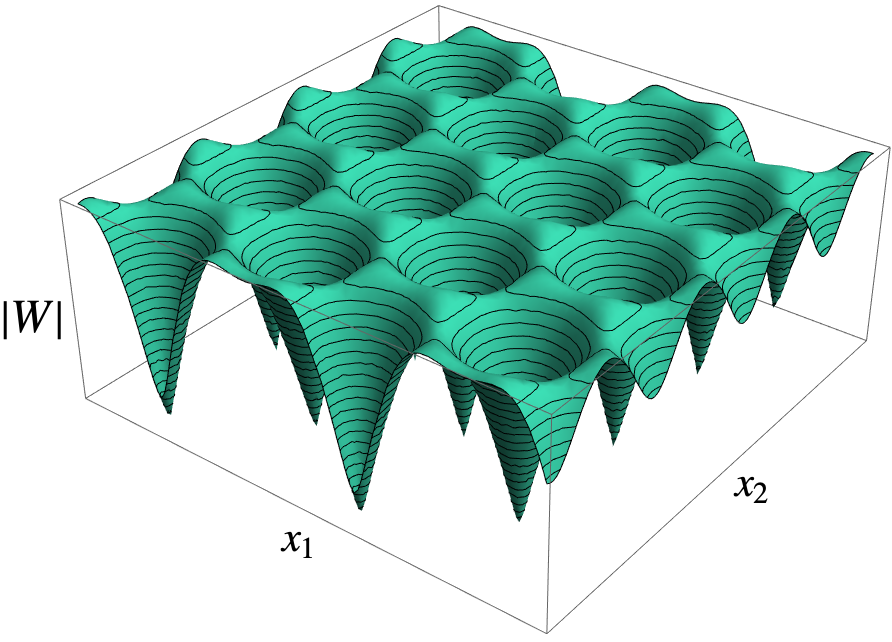
\includegraphics[width=7cm, height=5cm]{wcondensatereal.png}
        \caption{}
        \label{fig:W condensate abs}
    \end{subfigure}
    \hfill
    \begin{subfigure}[t]{0.45\textwidth}
        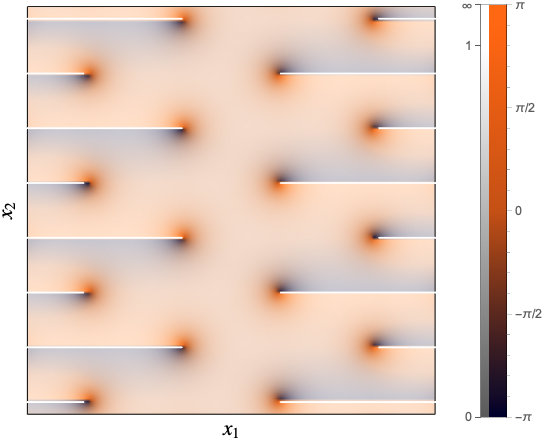
\includegraphics[width=6cm, height=5cm]{phaseplotWcondensate.png}
        \caption{}
        \label{fig:W condensate phase}
    \end{subfigure}
    \caption{\textit{Αριστερά: Η πλάτος $|W|$ ως συνάρτηση στο κάθετο στο μαγνητικό πεδίο επίπεδο. Οι ρίζες του πλάτους αντιστοιχούν στα κέντρα των εξαγωνικών δινών. Δεξιά: Το γράφημα της φάσης $\rm{Arg}(W)$, με βάση βαθμονομημένη χρωματική κλίμακα. Διαμέσου των φωτεινών ευθειών εκδηλώνεται ασυνέχεια $2\pi$ στη φάση. Οι ευθείες έχουν άκρο σε ρίζα του πλάτους και καταλήγουν στο άπειρο.}}
\end{figure}
\end{english}
\\

Εκτελώντας το μετασχηματισμό βαθμίδας
\begin{equation}\label{gauge tran in terms of the phase of W}
    A\subscr{\mu}\,\rightarrow\,A\subscr{\mu}+\frac{1}{e}\partial\subscr{\mu}\chi
\end{equation}
απαλείφεται η φάση του δυναμικού $W=|W|e\superscr{i\chi}$. 
%εντός της εξίσωσης \eqref{de for W condensation function}, και %με αντικατάσταση της \eqref{equation for Zi}, 
Τότε το ηλεκτρομαγνητικό δυναμικό $A\subscr{\mu}$ δίνεται συναρτήσει των πραγματικών ποσοτήτων $|W|,\phi$ από την έκφραση \cite{ambjornTheoryAndApplications,AMBJORN1990193}
\begin{equation}
    A\subscr{i}=\frac{1}{e}\epsilon\subscr{ij}\partial\subscr{j}(\ln|W|+2\cos\superscr{2}\theta\subscr{w}\ln\phi)\qquad i=1,2
\end{equation}
και δεν εκδηλώνει ασυνέχειες, σε αντίθεση με τη φάση $\rm{Arg}(W)=\chi$. 
Συνεπώς, σε ένα κλειστό επικαμπύλιο ολοκλήρωμα, που περιβάλλει τμήματα των ευθειών ασυνέχειας της φάσης, συνεισφέρει μόνο ο δεύτερος όρος της \eqref{gauge tran in terms of the phase of W}
\begin{equation}
    \oint (A\subscr{\mu}+\partial\subscr{\mu}\chi)dx\superscr{\mu}=\oint\partial\subscr{\mu}\chi dx\superscr{\mu}
\end{equation}
Η μαγνητική ροή διαμέσου της επιφάνειας Σ που περιβάλλεται από το βρόχο είναι κβαντισμένη και ισούται με 
%το επικαμπύλιο ολοκλήρωμα του ηλεκτρομαγνητικού δυναμικού, από %το οποίο όμως επιζεί μόνο ο προαναφερόμενος όρος
\begin{equation}\label{quantised magnetic flux}
    \int\limits_{\Sigma}F\subscr{12}d\superscr{2}x \,\,=\,\, n\Phi\subscr{o}\,\,=\,\, \oint\partial\subscr{\mu}\chi dx\superscr{\mu}
\end{equation}
όπου $n\in\mathbb{Z}$ και $\Phi\subscr{o}\equiv \frac{2\pi}{e}$ η στοιχειώδης μαγνητική ροή. Η διαφορά φάσης, που προκύπτει εκτελώντας το κλειστό επικαμπύλιο ολοκλήρωμα, είναι κβαντισμένη.\\
%επιτρέποντας την αντιστοιχία 

Αντιπαραβάλλουμε τα αποτελέσματα αυτά με τη συμπεριφορά υπεραγώγιμων υλικών εντός μαγνητικού πεδίου. 
%Συγκεκριμένα, οι περιοχές γύρω από τις οποίες το κλειστό %επικαμπύλιο ολοκλήρωμα είναι μη μηδενικό, είναι σε κοντινή %αναλογία με τις
Οι δίνες του συμπυκνώματος ζευγών Cooper σε υπεραγώγιμα υλικά απαγορεύουν τη διείσδυση στο υλικό εξωτερικού μαγνητικού πεδίου - φαινόμενο Meissner. Αντίθετα, οι δίνες του συμπυκνώματος μποζονίων $W$ ενισχύουν το αβελιανό μαγνητικό πεδίο $F\subscr{12}$, όπως φαίνεται από το θετικό πρόσημο της συνεισφοράς του συμπυκνώματος στην \eqref{equation for f12}.\\

Αυξάνοντας ακόμη περισσότερο το μαγνητικό πεδίο, 
%έξω από την περιοχή 
$F\subscr{12}\,>\,m\subscr{w}\superscr{2}$, το συμπύκνωμα διατηρεί την περιοδική μορφή του, \eqref{w condensate solution}, όπως μπορεί να αποδειχθεί διαταρακτικά 
%Η ύπαρξη των περιοδικών λύσεων 
\cite{ambjornTheoryAndApplications,AMBJORN1990193}. %αποδεικνύεται από τους Ambjorn και Olesen διαταρακτικά. 
%Η ανάλυση και τα αποτελέσματα τους είναι ανεξάρτητα των λύσεων %αυτών καθαυτών, αλλά, βασίζονται στην περιοδικότητα των |W| και %$\phi$ 
Εντός μιας κυψελίδας ικανοποιούνται οι εξισώσεις (στη βαθμίδα \eqref{gauge tran in terms of the phase of W})
\begin{english}
\begin{subequations}\label{coupled de for W and phi}
    \begin{equation}
        \partial\superscr{2}\ln|W|=-\frac{g\superscr{2}\phi\superscr{2}}{2}-2g\superscr{2}|W|\superscr{2}\qquad\partial\superscr{2}\equiv\partial\subscr{1}\superscr{2}+\partial\subscr{2}\superscr{2}
    \end{equation}
    \begin{equation}\label{de for phi2}
        \partial\superscr{2}\ln\phi\superscr{2}=\frac{g\superscr{2}}{2\cos\superscr{2}\theta\subscr{w}}(\phi\superscr{2}-v\superscr{2})+2g\superscr{2}|W|\superscr{2}
    \end{equation}
\end{subequations}
\end{english}
%Με χρήση των εξισώσεων \eqref{coupled de for W and phi}, χωρίς %να λυθούν αναλυτικά, 
Με βάση τις εξισώσεις αυτές, βρίσκουμε τη μέση τιμή ${\scriptstyle\left<\phi\superscr{2}\right>}$, ως προς την επιφάνεια $A$ μιας κυψελίδας
\begin{equation}
    \left<\phi\superscr{2}\right> \equiv \frac{1}{A}\int\subscr{A}\phi\superscr{2}d\superscr{2}x
\end{equation}
%Λόγω της θετικότητας και περιοδικότητας του $\phi\superscr{2}$, 
Oλοκληρώνοντας την \eqref{de for phi2}, η συνεισφορά του αριστερού μέλους στη μέση τιμή μηδενίζεται
\begin{equation}
    \int\subscr{A}\partial\superscr{2}\ln\phi\superscr{2}\,\,d\superscr{2}x=0
\end{equation}
Το ολοκλήρωμα της \eqref{equation for f12} και 
η εξίσωση \eqref{quantised magnetic flux} οδηγούν στη σχέση
%, δείνουν για το δεύτερο όρο τη μέση τιμή
\begin{equation}
    \frac{1}{A}\int\subscr{A}|W|\superscr{2}\,\,d\superscr{2}x=\frac{e\overline{F\subscr{12}}-m\subscr{W}\superscr{2}}{2e\superscr{2}}\qquad\overline{F\subscr{12}}\equiv\frac{2\pi n}{eA}
\end{equation}
όπου $\overline{F\subscr{12}}$ η μέση τιμή του μαγνητικού πεδίου ως προς την κυψελίδα. Εάν συνδυάσουμε τις πιο πάνω εξισώσεις, παίρνουμε 
%των παραπάνω δείνει 
\begin{equation}\label{expectation of higgs squared in a cell of periodicity}
    \left<\phi\superscr{2}\right>=v\superscr{2}\left( \frac{m\subscr{h}\superscr{2}}{m\subscr{h}\superscr{2}\sin\superscr{2}\theta\subscr{w}}-\frac{2e\cos\superscr{2}\theta\subscr{w}\overline{F\subscr{12}}}{v\superscr{2}g\superscr{2}\sin\superscr{2}\theta\subscr{w}} \right)\,\,=\,\,v\superscr{2}\, \frac{m\subscr{h}\superscr{2}-e\overline{F\subscr{12}}}{m\subscr{h}\superscr{2}-m\subscr{W}\superscr{2}},\qquad \overline{F\subscr{12}}\le \frac{m\subscr{h}\superscr{2}}{e}
\end{equation}

\section{Αποκατάσταση συμμετρίας}
Σύμφωνα με την \eqref{expectation of higgs squared in a cell of periodicity}, η μέση τιμή ${\scriptstyle\left<\phi\superscr{2}\right>}\rightarrow 0$ καθώς ${\scriptstyle e\overline{F\subscr{12}}}\rightarrow m\subscr{h}\superscr{2}$, και συνεπώς η αναμενόμενη τιμή του Higgs ελαττώνεται, ${\scriptstyle\left<\phi\right>\,}\rightarrow 0$. Στο στάδιο αυτό, συνεχίζει να εκδηλώνεται η ρήξη της ηλεκτρασθενούς συμμετρίας, αφού το πεδίο Higgs έχει μη μηδενική αναμενόμενη τιμή. Όταν ${\scriptstyle\left<\phi\superscr{2}\right>\,}=0$, η ρήξη της συμμετρίας παύει να υφίσταται, επειδή η αναμενόμενη τιμή ${\scriptstyle\left<\phi\right>\,}=0$ είναι συμμετρική ως προς τις συμμετρίες $SU(2)\,\times\,U(1)$. Η σχέση \eqref{expectation of higgs squared in a cell of periodicity}
%, αδυνατεί να διευκρινήσει την κατάσταση του μοντέλου για τιμές %${\scriptstyle e\overline{F\subscr{12}}\;\;\ge\;\;} %m\subscr{h}\superscr{2}$. 
σηματοδοτεί τη μετάβαση στην συμμετρική φάση της ηλεκτρασθενούς θεωρίας, με τα πεδία βαθμίδας να είναι τα τρία μη αβελιανά $W\superscr{i}\subscr{\mu}$ και το αβελιανό $B\subscr{\mu}$. Υπενθυμίζουμε τις σχέσεις και τους αντίστοιχους τανυστές έντασης, \eqref{tensors for electroweak gauge fields}:
\begin{english}
\begin{subequations}
    \begin{equation}
        B\subscr{\mu}=\cos\theta\subscr{w}\, A\subscr{\mu}-\sin\theta\subscr{w}\, Z\subscr{\mu}
    \end{equation}
    \begin{equation}
        W\superscr{3}\subscr{\mu}=\sin\theta\subscr{w} A\subscr{\mu}+\cos\theta\subscr{w} Z\subscr{\mu}
    \end{equation}
    \begin{equation}
        W\subscr{\mu}\superscr{1}=\frac{1}{\sqrt{2}}(W\subscr{\mu}+W\subscr{\mu}\superscr{\dagger})\qquad W\subscr{\mu}\superscr{2}=\frac{i}{\sqrt{2}}(W\subscr{\mu}-W\subscr{\mu}\superscr{\dagger})
    \end{equation}
  \begin{equation}
      B\subscr{\mu\nu}\,=\,\partial\subscr{\mu}B\subscr{\nu}-\partial\subscr{\nu}B\subscr{\mu}
  \end{equation}
  \begin{equation}
      G\superscr{i}\subscr{\mu\nu}\,=\,\partial\subscr{\mu}W\superscr{i}\subscr{\nu}-\partial\subscr{\nu}W\superscr{i}\subscr{\mu}+g\epsilon\superscr{ijk}W\superscr{j}\subscr{\mu}W\superscr{k}\subscr{\nu}
  \end{equation}
\end{subequations}
\end{english}
Η συμμετρική ως προς $SU(2)\,\times\,U(1)$ λαγκραντζιανή είναι
\begin{equation}
    \mathcal{L}=-\frac{1}{4}G\subscr{\mu\nu}\superscr{i}G\superscr{i\,\mu\nu}-\frac{1}{4}B\subscr{\mu\nu}B\superscr{\mu\nu}+|D\subscr{\mu}\phi|\superscr{2}-\lambda(\phi\superscr{2}-v\superscr{2})\superscr{2}
\end{equation}
\\

Mε βάση τις εξισώσεις \eqref{ansatz for W field}, \eqref{equation for f12}, \eqref{equation for Z12}, συμπεραίνουμε ότι, στο διάστημα ${\scriptstyle m\subscr{W}\superscr{2}\;\;\le\;\; e\overline{F\subscr{12}}\;\;\le\;\;m\subscr{h}\superscr{2}}$, οι μόνες μη μηδενικές μαγνητικές εντάσεις είναι οι ακόλουθες
\begin{english}
\begin{subequations}
\begin{equation}
    B\subscr{12}=\frac{g\,v\superscr{2}}{2\tan\theta\subscr{w}}+\frac{g}{2}\tan\theta\subscr{w}(v\superscr{2}-\phi\superscr{2})
\end{equation}
\begin{equation}
    G\subscr{12}\superscr{3}=-G\subscr{21}\superscr{3}=\frac{1}{2}g\superscr{2}\phi\superscr{2}
\end{equation}
\end{subequations}
\end{english}
Επομένως, καθώς ${\scriptstyle e\overline{F\subscr{12}}}\rightarrow m\subscr{h}\superscr{2}$, επιβιώνει μόνο το αβελιανό μαγνητικό πεδίο που συνδέεται με το υπερφορτίο $U(1)\subscr{Y}$. Συγκεκριμένα, το μαγνητικό αυτό πεδίο είναι παράλληλο με το αρχικό ηλεκτρομαγνητικό πεδίο  $U(1)\subscr{EM}$. Επειδή οι εντάσεις $G\superscr{i}\subscr{\mu\nu}$ μηδενίζονται, μηδενίζεται το μη αβελιανό μαγνητικό πεδίο $SU(2)$. 
%συνεπάγεται ότι τα πεδία $W\superscr{i}\subscr{\mu}$ δεν έχουν %κινητικούς όρους και έτσι μπορούν να απαλειφθούν από τη %λαγκρατζιανή με μετασχηματισμούς βαθμίδας. Το μαγνητικό πεδίο %λοιπόν, γίνεται εξολοκλήρου U(1)$\subscr{Y}$ ενώ 
H $SU(2)$ συνειστώσα του αρχικού ηλεκτρομαγνητικού πεδίου θωρακίζεται. Το υπερμαγνητικό πεδίο ισούται με 
\begin{equation}\label{hypermagnetic field ge to higgs mass}
    g\subscr{\y}B\subscr{12}\ge m\subscr{h}\superscr{2}\equiv 4\lambda v\superscr{2}\quad(=2\mu\superscr{2})
\end{equation}
\\

Η λαγκραντζιανή που περιγράφει τη σύζευξη του αβελιανού πεδίου βαθμίδας U(1)$\subscr{Y}$ και του βαθμωτού πεδίου Higgs 
%και της σύζευξης τους 
είναι
\begin{equation}
    \mathcal{L}=-B\subscr{\mu\nu}\superscr{2}+\underbrace{|(\partial\subscr{\mu}-i\frac{1}{2}g\subscr{\y}B\subscr{\mu})\phi|\superscr{2}+\mu\superscr{2}|\phi|\superscr{2}}\subscr{\mathcal{L}\subscr{o}}-\lambda(\phi\superscr{*}\phi)\superscr{2}-\lambda v\superscr{2},\qquad (\mu\superscr{2}=2\lambda v\superscr{2})
\end{equation}
όπου το υπερφορτίου του Higgs ισούται με $Y{\scriptstyle=\frac{1}{2}}$ και $g\subscr{\y}{\scriptstyle=} g\tan\theta\subscr{w}$ η σταθερά σύζευξης του U(1)$\subscr{Y}$ πεδίου βαθμίδας. Το δυναμικό $B\subscr{\mu}$ 
%πρέπει να ικανοποιεί τις εξισώσεις για σταθερό πεδίο στις %εγκάρσιες διευθύνσεις $x\subscr{1}-x\subscr{2}$
%\begin{equation}
%    \text{constant}=B\subscr{\mu\nu}=\partial\subscr{\mu}B\subs%cr{\nu}-\partial\subscr{\nu}B\subscr{\mu}
%\end{equation}
στη βαθμίδα Landau δίδεται από την έκφραση
\begin{equation}
    B\subscr{\mu}=x\subscr{1}B\subscr{12}\de\subscr{\mu 2}\qquad\left(\Rightarrow B\subscr{\mu}\superscr{2}=-(B\subscr{12}x\subscr{1})\superscr{2}\right)
\end{equation}
όπου $B\subscr{12}$ το σταθερό μαγνητικό πεδίο.
%Απομονώνοντας τους όρους $\mathcal{L}\subscr{o}$, 
Οι εξισώσεις κίνησης για το πεδίο Higgs, 
για $\phi \sim 0$ είναι
\begin{equation}\label{equations of motion for higgs around phi=0}
    \frac{\de \mathcal{L}\subscr{o}}{\de \phi\superscr{*}}-\partial\subscr{\mu}\frac{\de\mathcal{L}\subscr{o}}{\de(\partial\subscr{\mu}\phi\superscr{*})}=0\quad\Rightarrow\quad \partial\superscr{2}\phi=\left(-\frac{g\subscr{\y}\superscr{2}}{4}(B\subscr{12}x\subscr{1})\superscr{2}-ig\subscr{\y}B\subscr{\mu}\partial\subscr{\mu}+\mu\superscr{2}\right)\phi
\end{equation}
Χωρίζοντας μεταβλητές $\phi=e\superscr{iE\subscr{n}x\subscr{o}}\phi\subscr{n}(x\subscr{1},x\subscr{2},x\subscr{3})$, 
%η εξίσωση \eqref{equations of motion for higgs around phi=0} %γράφεται ως η εξίσωση ιδιοτιμών
παίρνουμε
\begin{equation}\label{eigenvalue equation from eom for higgs}
    E\subscr{n}\superscr{2}\phi\subscr{n}=-\left( \partial\superscr{2}\subscr{i} -g\subscr{\y}\superscr{2}\left(\frac{B\subscr{12}x\subscr{1}}{2}\right)\superscr{2}-ig\subscr{\y}(B\subscr{12}x\subscr{1})\partial\subscr{2}+\mu\superscr{2} \right)\phi\subscr{n}
\end{equation}
%Περαιτέρω απλοποίηση γίνεται, αναγνωρίζοντας ότι, 
Οι λύσεις πρέπει να είναι αναλλοίωτες ως προς μεταφορές στις διευθύνσεις $x\subscr{2},\,x\subscr{3}$. 
%αφού δεν εμφανίζονται στην εξίσωση ιδιοτιμών. 
Επομένως θέτουμε 
\begin{equation}
    \phi\subscr{n}\sim e\superscr{ip\subscr{2}x\subscr{2}}e\superscr{ip\subscr{3}x\subscr{3}}\Tilde{\phi}\subscr{n}(x\subscr{1})
\end{equation}
Η \eqref{eigenvalue equation from eom for higgs} παίρνει τη μορφή
\begin{equation}\label{eigenvalue equation from eom for higgs simplified}
    E\subscr{n}\superscr{2}\Tilde{\phi}\subscr{n}=\left(p\subscr{3}\superscr{2}-\mu\superscr{2}-\partial\subscr{1}\superscr{2}+\left(\frac{g\subscr{\y}B\subscr{12}}{2}x\subscr{1}-p\subscr{2}\right)\superscr{2}\right)\Tilde{\phi}\subscr{n}
\end{equation}
Οι τελευταίοι δύο όροι στα δεξιό μέλος της \eqref{eigenvalue equation from eom for higgs simplified} διαγονοποιούνται με χρήση των ιδιοσυναρτήσεων ενός αρμονικού ταλαντωτή στην διεύθυνση $x\subscr{1}$, συχνότητας $\frac{g\subscr{\y}B\subscr{12}}{2}$. Οι αντίστοιχες ιδιοτιμές είναι
\begin{equation}
    g\subscr{\y}B\subscr{12}\left( n+\frac{1}{2} \right)
\end{equation}
Ο ακέραιος αριθμός $n$ χαρακτηρίζει τις στάθμες Landau. Η ενέργεια της χαμηλότερης στάθμης είναι
\begin{equation}\label{higgs energy lowest landau level around phi=0}
    E\superscr{2}\subscr{o}=p\subscr{3}\superscr{2}-\mu\superscr{2}+\frac{g\subscr{\y}B\subscr{12}}{2}
\end{equation}
\\

Το υπερμαγνητικό πεδίο ικανοποιεί τη σχέση \eqref{hypermagnetic field ge to higgs mass} και άρα η ενεργός μάζα του πεδίου Higgs που απορρέει από την εξίσωση διασποράς \eqref{higgs energy lowest landau level around phi=0} είναι θετική. Επομένως, η συμμετρική κατάσταση ${\scriptstyle\phi=0}$ είναι ευσταθής όταν το μαγνητικό πεδίου παίρνει τιμές στο διάστημα \eqref{hypermagnetic field ge to higgs mass}. Η ηλεκτρασθενής συμμετρία επαναφέρεται.\\ 

Το υπερμαγνητικό πεδίο συζεύγνυται διαφορετικά με την ύλη. Αντικαθιστούμε τη %αλλαγές αντικατοπτρίζονται από την αντικατάσταση της 
σταθερά σύζευξης του ηλεκτρομαγνητισμού
\begin{equation}
    e\equiv \frac{gg\subscr{\y}}{\sqrt{g\superscr{2}+g\subscr{\y}\superscr{2}}},\qquad \left(g=\frac{g\subscr{\y}}{\tan\theta\subscr{w}}\right)
\end{equation}
με την υπερμαγνητική σταθερά σύζευξης, $e\rightarrow g\subscr{\y}=\frac{e}{\cos\theta\subscr{w}}$. Για παράδειγμα, η μάζα μιας ακραίας οπής ελαττώνεται κατά $\cos\theta\subscr{w}$:
\begin{equation}
    M\subscr{e}=\sqrt{\frac{\pi}{G}}\frac{Q}{e}\,\rightarrow\,\sqrt{\frac{\pi}{G}}\frac{Q}{g\subscr{\y}}=\sqrt{\frac{\pi}{G}}\frac{Q}{e}\cos\theta\subscr{w}
\end{equation}

\begin{comment}
\section*{Προχειρο}
Η συγκέντρωση επηρεάζει την αναμενόμενη τιμή του Higgs $\left<\phi\right>$ μεταξύ των κατωφλίων $m\subscr{w}\superscr{2}\le|F|\le m\subscr{h}\superscr{2}$ και παρουσιάζεται στο άρθρο συναρτήσει της αναμενόμενης τιμής $|\left<\phi\subscr{o}\right>|\equiv v$ του συνηθισμένου κενού
\begin{equation}
    |\left<\phi\right>|\superscr{2} = v\superscr{2}\frac{m\subscr{h}\superscr{2}-|F|}{m\subscr{h}\superscr{2}-m\superscr{2}\subscr{w}}.\qquad m\subscr{w}\superscr{2}\le|F|\le m\subscr{h}\superscr{2}
\end{equation}
Είναι εμφανές ότι, αν και το Higgs δεν αλληλεπιδρά ηλεκτρομαγνητικά, επηρεάζεται έμμεσα μέσω της αλληλεπίδρασης των spin-1 μποζονίων με το εξωτερικό μαγνητικό πεδίο. Οι φυσικές συνέπειες της αύξησης των spin-1 σωματιδίων επεκτείνονται και στο ίδιο το μαγνητικό πεδίο \cite{AMBJORN1990193,ambjornTheoryAndApplications}. Η ευσταθής λύση του πεδίου στο διάστημα $|F|\ge m\superscr{2}\subscr{h}$ ($r\le r\subscr{h}$) καταλήγει να είναι ένα καθαρά αβελιανό πεδίο $\text{U(1)}\subscr{Y}$. Με χρήση του συμβολισμού της ενότητας \ref{section local gauge theory}, όπου $G\superscr{i}\subscr{\mu\nu}$ και $B\subscr{\mu\nu}$ οι τανυστές που αντιστοιχούν στα πεδία βαθμίδας της συμμετρικής φάσης της ηλεκτρασθενούς θεωρίας $SU(2)\times U(1)$, οι ευσταθείς λύσεις είναι \cite{AMBJORN1990193,ambjornTheoryAndApplications}
\begin{equation}
    \left<\phi\right>\rightarrow 0\,\Rightarrow\,\left\{ \begin{array}{l} G\superscr{i}\subscr{\mu\nu} \sim \left<\phi\right> \rightarrow 0 \\ B\subscr{\mu\nu}\ne 0 \end{array} \right.
\end{equation}
Μέσω του υπερφορτίου ½, το πεδίου Higgs συζεύγνυται με το πλέον υπερμαγνητικό πεδίο και η ενέργεια του αναβαθμίζεται με τη συνεισφορά του επιπέδου Landau. Για το χαμηλότερο επίπεδο n=0, το υπερμαγνητικό πεδίο συνεισφέρει θετικά στην ενεργό μάζα του πεδίου και αποδίδει ένα θετικό τετραγωνικό ως προς το πεδίο όρο εντός του ενεργού δυναμικού
\begin{equation}
    V(\phi\superscr{\dagger}\phi)\,=\, (-\mu\superscr{2}+\frac{|F|}{2})\,|\phi|\superscr{2}+\lambda|\phi|\superscr{4}
\end{equation}
Όπως αναφέρθηκε στην προηγούμενη ενότητα, πέραν της κρίσιμης τιμής της έντασης $|F|\ge 2\mu\superscr{2}\equiv m\superscr{2}\subscr{h}$ ($r\le r\subscr{h}$) το δυναμικό ελαχιστοποιείται μόνο από πεδίο με μέση τιμή $\left<\phi\right>=0$ και επομένως η ευσταθής πλέον κατάσταση είναι αυτή με την αποκατάσταση της συμμετρία. το διάστημα $r<r\subscr{h}$, είναι επακόλουθο ότι 
\end{comment}

\section{Καταστολή μηχανισμού Higgs}
Η αναμενόμενη τιμή του πεδίου Higgs ελαττώνεται καθώς αυξάνεται η ένταση του μαγνητικού πεδίου μέχρι να μηδενιστεί εντελώς στην περιοχή $r\subscr{e}\le r \le r\subscr{h}$. Οι μάζες των φερμιονίων μηδενίζονται.
%σωματιδίων ύλης (επακόλουθο της σύζευξης με το πεδίο $\phi$ %στην ενότητα \ref{section mass for fermions} και του ασύμετρου %κενού) είναι ανάλογες της συνήθης μέσης τιμής %$\left<\phi\right>\ne 0$, αναμένεται να μηδενιστούν. Η μάζα των %φερμιονικών πεδίων (μέσω του μηχανισμού Higgs) καταστέλλεται, %και τα πεδία καθιστώνται άμαζα εντός του καθορισμένου %διαστήματος. 
Έτσι, γίνονται πιο έντονες οι κβαντικές διακυμάνσεις των πεδίων αυτών και ενισχύεται το φαινόμενο της
%Κβαντικές διακυμάνσεις φερμιονικών πεδίων κοντά στον ορίζοντα %της μελανής οπής οδηγούν σε 
%Τα φερμιονικά πεδία θετικής ενέργειας που διαδίδονται προς το %εξωτερικό της κορώνας με την ταχύτητα του φωτός (μέχρι να %αποκτήσουν ξανά μάζα εκτός της κορώνας), συνεισφέροντας στην 
ακτινοβολίας Hawking. Στην ενίσχυση της ακτινοβολίας συνεισφέρει ο εκφυλισμός της χαμηλότερης στάθμης Landau,
%. Ο εκφυλισμός του ενεργειακού επιπέδου διαφέρει ελαφρώς από %αυτόν της ενότητας \ref{section LLL degeneracy} αλλά %εξακολουθεί 
ο οποίος είναι ανάλογος του μαγνητικού φορτίου Q. 
%Η διαφορά οφείλεται στο κλασματικό υπερφορτίο των φερμιονικών %πεδίων. 

\section{Υπερφορτίο και εκφυλισμός}
Στην ενότητα \ref{section LLL degeneracy}, προσδιορίσαμε τον εκφυλισμό της χαμηλότερης στάθμης Landau LLL για σωματίδια με φορτίο ίσο με ακέραιου πολλαπλάσιο του φορτίου του ηλεκτρονίου. %Ο εκφυλισμός του LLL της ενότητας \ref{section LLL degeneracy} %αναθεωρείται 
Στην περίπτωση υπερμαγνητικού πεδίου, όπως συμβαίνει εντός της ηλεκτρασθενούς κορώνας, θα πρέπει να λάβουμε υπόψη το υπερφορτίο κάθε σωματιδίου. 
%αναπαράστασης της SU(3)$\times$SU(2)$\times$U(1) ομάδας. 
Τα υπερφορτία φαίνονται στον πίνακα \ref{tab:table with particles and su3, su2 representations}. 
%Πέραν του εκφυλισμού, 
%Θα εξετάσουμε επίσης τη συμπεριφορά φερμιονικών πεδίων 
%εντός του συνδυασμού υπερμαγνητικού και βαρυτικού πεδίου έξω %από 
στην εξωτερική περιοχή μιας μελανής οπής. Στην επόμενη ενότητα μελετούμε τις λύσεις της εξίσωσης Dirac στην παρουσία βαρυτικού και ηλεκτρομαγνητικού πεδίου.

\section{Εξίσωση Dirac}\label{section dirac equation in gravity}
Η γενίκευση της εξίσωσης Dirac σε καμπύλους χώρους γίνεται με την χρήση κατάλληλης συναλλοίωτης παραγώγου. Αυτή ορίζεται ως ακολούθως 
%απαίτηση για παραγώγους σπινορικών πεδίων με τανυστικούς %μετασχηματισμούς οδηγεί στον ορισμό
\begin{equation}
    \nabla\subscr{\mu}\,\equiv\,\partial\subscr{\mu}+\frac{1}{4}\omega\subscr{\mu ab}\gamma\superscr{a}\gamma\superscr{b}
\end{equation}
όπου $\omega\subscr{ab\mu}$ η σπινορική σύνδεση (spin connection) \cite{Carroll2003-CARSAG-3}
\begin{equation}\label{spin connection}
    \omega\subscr{\mu ab}\,\equiv\,e\subscr{\nu a}e\superscr{\lambda}\subscr{\;\;b}\Gamma\superscr{\nu}\subscr{\mu\lambda}-e\superscr{\lambda}\subscr{\;\;b}\,\partial\subscr{\mu}e\subscr{\lambda a}
\end{equation}
και $\gamma\superscr{a}$ οι πίνακες Dirac 
%του επίπεδο χώρου Minkowski 
με τις αντιμεταθετικές σχέσεις 
\begin{equation}\label{gamma anticommutator 4d}
    \{ \gamma\superscr{a},\gamma\superscr{b} \}\,=\,2\,\mink[1]{a}{b}\,\mathbf{I\subscr{4}}
\end{equation}
%και οι τετράδες (vierbein) διανυσματικών πεδίων (ένα για κάθε %τιμή του δείκτη $a$) 
Τα πεδία $e\subscr{\mu}\superscr{\;\;a}$ συνδέονται με τη μετρική
%καθορίζουν εφαπτόμενες ορθοκανονικές βάσεις σε κάθε σημείο της %πολλαπλότητας με την μετρική 
$\g{\mu}{\nu}$ με βάση τη σχέση \cite{Carroll2003-CARSAG-3}
\begin{equation}
    \g{\mu}{\nu}=e\subscr{\mu}\superscr{\;\;a}e\subscr{\nu}\superscr{\;\;b}\mink{a}{b},\qquad \mink{a}{b}:=\text{diag}(-1,+1,+1,+1)
\end{equation}
%καθώς επίσης ισχύει η εξής διαφοροποίηση στους κανόνες που %ακολουθούν 
Οι λατινικοί και οι ελληνικοί δείκτες ανεβοκατεβαίνουν ως εξής
\begin{equation}\label{vierbein identity manipulating indices}
    e\superscr{\mu}\subscr{\;\;a}=\g[1]{\mu}{\nu}\mink{a}{b}e\superscr{\;\;b}\subscr{\nu}
\end{equation}
\\

Όταν το φερμιονικό πεδίο αλληλεπιδρά με ένα 
%φορτισμένου (q) σπινορικού πεδίου με 
ηλεκτρομαγνητικό πεδίο 
%\eqref{vector potential for monopole in curvilinear coo} όπου %$Q=2s\subscr{o}$ είναι το ακέραιο μαγνητικό φορτίο
%\begin{equation}
%    A\subscr{\mu}=\frac{s\subscr{o}}{e}\cos\theta\,\,\de\subscr%{\mu\phi}
%\end{equation}
%εγκαθίσταται στον ορισμό της 
η πιο πάνω συναλλοίωτη παράγωγος ανάγεται στην 
%με το συνηθισμένο τρόπο
\begin{equation}
    D\subscr{\mu}\,\equiv\,\partial\subscr{\mu}+\frac{1}{4}\omega\subscr{\mu ab}\gamma\superscr{a}\gamma\superscr{b}+iqA\subscr{\mu}
\end{equation}
Η εξίσωση Dirac για άμαζο φερμιονικό πεδίο $\chi$ είναι
\begin{equation}\label{general dirac equation}
    ie\superscr{\mu}\subscr{\;\;a}\gamma\superscr{a}D\subscr{\mu}\chi=0
\end{equation}
\\

Γράφουμε τη μετρική \eqref{ReissnerNordmetric} στη βοηθητική μορφή
\begin{equation}
    ds\superscr{2}\,=\,F(r)\left( -dt\superscr{2}+dx\superscr{2} \right)+r\superscr{2}(x)d\Omega\superscr{2}\,,\qquad F(r)=\left(1-\frac{2G M}{r}+\frac{G\pi Q^2}{e^2r^2}\right)
\end{equation}
%με την αντικατάσταση της ακτινικής συνεταγμένης r
όπου
\begin{equation}
    dx\,\equiv\,\frac{dr}{F(r)}
\end{equation}
%Το γωνιακό κομμάτι της μετρικής έχει τον συντελεστή %$r\superscr{2}$ ως προς τον οποίο παραγοντοποιείται η μετρική. %Ο καθολικός θετικός παράγοντας της μετρικής είναι ένας τοπικός %παράγοντας επανακλιμάκωσης (Weyl transformation) της μετρικής %και επιτρέπεται να αγνοηθεί αφού 
Η άμαζη εξίσωση Dirac είναι αναλλοίωτη ως προς τοπικούς σύμμορφους μετασχηματισμούς Weyl. Για τον λόγο αυτό, μπορούμε να αμελήσουμε έναν ολικό σύμμορφο παράγοντα, θέτοντας το συντελεστή του γωνιακού μέρους της μετρικής ίσο με τη μονάδα: 
%Το γωνιακό κομμάτι της μετρικής είναι πλέον ανεξάρτητο των t %και x
\begin{equation}\label{metric with a weyl factor for the t-x part}
     ds\superscr{2}\,=\,e\superscr{2\rho}\left( -dt\superscr{2}+dx\superscr{2} \right)+d\Omega\superscr{2},\qquad  e\superscr{2\rho(x)}\equiv\frac{F(r)}{r\superscr{2}}
\end{equation}
Με βάση τη μετρική \eqref{metric with a weyl factor for the t-x part}, οι μη μηδενικές συνιστώσες του πεδίου $e\superscr{\;\;a}\subscr{\mu}$ είναι
\begin{equation}
    e\superscr{\;\;0}\subscr{t}=e\superscr{\,\rho},\quad  e\superscr{\;\;1}\subscr{x}=e\superscr{\,\rho},\quad
    e\superscr{\;\;2}\subscr{\theta}=1,\quad
    e\superscr{\;\;3}\subscr{\theta}=\sin\theta
\end{equation}
Βρίσκουμε στη συνέχεια τα μη μηδενικά στοιχεία της σπινορικής σύνδεσης \eqref{spin connection}
\begin{equation}
    \omega\subscr{t10}=-\omega\subscr{t01}=\frac{d\rho}{dx}\equiv\rho',\quad\omega\subscr{\phi32}=-\omega\subscr{\phi23}=\cos\theta
\end{equation}
Στον δισδιάστατο χωρόχρονο $tx$, οι πίνακες Dirac ικανοποιούν τις αντιμεταθετικές σχέσεις
\begin{equation}
    \{ \bar{\gamma}\superscr{a},\bar{\gamma}\superscr{b} \}\,=\,2\,\mink[1]{a}{b}\,\mathbf{I\subscr{2}},\qquad \mink{a}{b}:=\text{diag}(-1,+1)
\end{equation}
που ικανοποιούνται από τους πίνακες 
\begin{equation}\label{gamma 2d repre t-x}
    \bar{\gamma}\superscr{0}=i\sigma\superscr{x}\qquad\bar{\gamma}\superscr{1}=\sigma\superscr{\y}
\end{equation}
Για τη σφαίρα, οι αντίστοιχες σχέσεις είναι
\begin{equation}
     \{ \bar{\gamma}\superscr{a},\bar{\gamma}\superscr{b} \}\,=\,2\,\de\superscr{ab}\,\mathbf{I\subscr{2}},\qquad \de\superscr{ab}:=\text{diag}(+1,+1)
\end{equation}
και
\begin{equation}\label{gamma 2d repre theta-phi}
    \bar{\gamma}\superscr{1}=\sigma\superscr{x}\qquad\bar{\gamma}\superscr{2}=\sigma\superscr{\y}
\end{equation}
Οι δυσδιάστατες αναπαραστάσεις, \eqref{gamma 2d repre t-x} και \eqref{gamma 2d repre theta-phi}, συνδυάζονται στις ακόλουθες τετραδιάστατες \cite{Maldacena2018TraversableWI} 
\begin{equation}\label{gamma 4d repre}
    \gamma\superscr{0} = i\sigma\superscr{x}\otimes\mathbf{I}\subscr{2}\qquad
    \gamma\superscr{1} = \sigma\superscr{\y}\otimes\mathbf{I}\subscr{2}\qquad
    \gamma\superscr{2} = \sigma\superscr{z}\otimes\sigma\superscr{x}\qquad
    \gamma\superscr{3} = \sigma\superscr{z}\otimes\sigma\superscr{\y}
\end{equation}
που ικανοποιούν τις σχέσεις \eqref{gamma anticommutator 4d}.
Στην αναπαράσταση \eqref{gamma 4d repre} ο  χειραλικός τελεστής %χειραλικότητας ορίζεται ως το εξωτερικό γινόμενο
είναι
\begin{equation}\label{gamma 5 repre in 4d}
    \gamma\superscr{5}=i\gamma\superscr{0}\gamma\superscr{1}\gamma\superscr{2}\gamma\superscr{3}=i(-\sigma\superscr{z}\otimes i\sigma\superscr{z})=\sigma\superscr{z}\otimes\sigma\superscr{z}
\end{equation}
Οι λύσεις της \eqref{general dirac equation} αποτελούν ιδιοκαταστάσεις του \eqref{gamma 5 repre in 4d} με ιδιοτιμές +1 και -1, και αντιστοιχούν σε δεξιόστροφα και αριστερόστροφα φερμιονικά πεδία. Αντικαθιστώντας τα πιο πάνω στην \eqref{general dirac equation}, η εξίσωση Dirac παίρνει τη μορφή
\begin{equation}
    \left[e\superscr{-\rho}\left(i\sigma\superscr{x}\partial\subscr{t}+\sigma\superscr{\y}(\partial\subscr{x}+\frac{\rho'}{2})\right)\otimes \mathbf{I}\subscr{2} \;+\; \sigma\superscr{z}\otimes\left( \sigma\superscr{\y}\frac{\partial\subscr{\phi}+iqA\subscr{\phi}}{\sin\theta} + \sigma\superscr{x}\left(\partial\subscr{\theta}+\frac{\cot\theta}{2}\right) \right) \right]\chi=0
\end{equation}
Υπενθυμίζουμε ότι στην περίπτωση μαγνητικού μονοπολικού πεδίου η μόνη μη μηδενική συνιστώσα του δυναμικού είναι η $A_\phi$.

\section{Λύσεις Dirac}\label{sec:dirac solutions in magnetic mon field}
Οι τετραδιάστατες λύσεις της εξίσωσης \eqref{general dirac equation} σε χωροχρόνο της μορφής $\mathbf{M}=\mathbb{R}\superscr{1,1}\times S\superscr{2}$ ανάγονται σε τανυστικό γινόμενο δύο δισδιάστατων σπινόρων $\psi$ και $\eta$ \cite{Maldacena2018TraversableWI}
\begin{equation}\label{dirac solution ansatz}
    \chi\subscr{ij}(t,x,\theta,\phi)\,=\,e\superscr{-\rho(x)}\psi\subscr{i}(t,x)\otimes\eta\subscr{j}(\theta,\phi),\qquad i,j=1,2
\end{equation}
%Εφαρμόζοντας το ansatz \eqref{dirac solution ansatz} 
Η εξίσωση Dirac ανάγεται σε σύστημα δύο ασύζευκτων διαφορικών εξισώσεων
\begin{english}
\begin{subequations}
  \begin{equation}
    \label{dirac t-x de}
    \left[i\sigma\superscr{x}\partial\subscr{t}+\sigma\superscr{\y}\partial\subscr{x}\right]\psi=0
  \end{equation}
  \begin{equation}
    \label{dirac θ-φ de}
        \left[\sigma\superscr{\y}\frac{\partial\subscr{\phi}+iqA\subscr{\phi}}{\sin\theta} + \sigma\superscr{x}\left(\partial\subscr{\theta}+\frac{\cot\theta}{2}\right)\right]\eta=0
  \end{equation}
\end{subequations}
\end{english}
Οι δύο εξισώσεις της \eqref{dirac θ-φ de}, μια για κάθε συνιστώσα του σπίνορα $\eta$, 
\begin{equation}
    \eta\,:=\,\left( \begin{array}{c} \eta\subscr{1}\\ \eta\subscr{2} \end{array} \right)
\end{equation}
ικανοποιούνται με χρήση των ιδιοκαταστάσεων Haldane \eqref{monomial eigenfunction}. Για φερμιονικό πεδίο με θετικό φορτίο $q=e$, η λύση είναι
\begin{equation}
    \eta\subscr{+}\equiv\left( \begin{array}{c} \eta\subscr{1}\\ 0 \end{array} \right),\qquad\quad
    \eta\subscr{1}= \left(\cos\frac{\theta}{2}\right)\superscr{s\subscr{o}-\frac{1}{2}+m}\left(\sin\frac{\theta}{2}\right)\superscr{s\subscr{o}-\frac{1}{2}-m}e\superscr{- im\phi}
\end{equation}
Για αρνητικό φορτίο $q=-e$ παίρνουμε
\begin{equation}
    \eta\subscr{-}\equiv\left( \begin{array}{c} 0\\ \eta\subscr{2} \end{array} \right),\qquad\quad
    \eta\subscr{2}= \left(\cos\frac{\theta}{2}\right)\superscr{s\subscr{o}-\frac{1}{2}+m}\left(\sin\frac{\theta}{2}\right)\superscr{s\subscr{o}-\frac{1}{2}-m}e\superscr{im\phi}
\end{equation}
Οι σπίνορες αυτοί έχουν καλά ορισμένη χειραλικότητα, $\sigma\superscr{z}\eta\subscr{\pm}=\pm\eta\subscr{\pm}$, όπως φένεται από τη δράση του τελεστή χειραλικότητας 
στην αναπαράσταση της σφαίρας $S\superscr{2}$, $\mathbf{I\subscr{2}}\otimes\sigma\superscr{z}$. Αρνητικά (θετικά) φορτισμένα φερμιονικά πεδία περιγράφονται με βάση τον σπίνορα $\eta\subscr{-}$ ($\eta\subscr{+}$). 
%σπίνορα στη σφαίρα $S\superscr{2}$. 
Για πεδία με κλασματικό φορτίο η ανάλυση είναι ποιοτικά παρόμοια.\\

%με διαφορά στον εκφυλισμό των ιδιοκαταστάσεων Haldane. 
Η ανάλυση της εξίσωσης \eqref{dirac t-x de} γίνεται με παρόμοιο τρόπο. Συναρτήσει των συνιστωσών του $\psi$, η \eqref{dirac t-x de} ανάγεται στις
\begin{english}
\begin{subequations}
  \begin{equation}
    \label{t-x de for psi1}
        \left( \partial\subscr{t}+\partial\subscr{x} \right)\psi\subscr{1}=0
    \end{equation}
  \begin{equation}
    \label{t-x de for psi2}
        \left( \partial\subscr{t}-\partial\subscr{x} \right)\psi\subscr{2}=0
  \end{equation}
\end{subequations}
\end{english}
%όπου φανερώνεται η μορφή των λύσεων
Οι λύσεις έχουν τη μορφή
\begin{english}
\begin{subequations}\label{dirac solutions t-x}
  \begin{equation}
    \label{t-x solution for psi1}
        \psi\subscr{1}:=\psi\subscr{1}(t-x)
    \end{equation}
  \begin{equation}
    \label{t-x solution for psi2}
        \psi\subscr{2}:=\psi\subscr{2}(t+x)
  \end{equation}
\end{subequations}
\end{english}
Η συνάρτηση \eqref{t-x solution for psi1} περιγράφει ένα δεξιόστροφο, εξερχόμενο πεδίο. 
%κινούμενο προς αύξουσες τιμές της συντεταγμένης x (r), επομένως %είναι δεξιοκίνητο και απομακρύνεται από τον ορίζοντα (out). 
Αντίθετα, η \eqref{t-x de for psi2} περιγράφει αριστερόστροφα, εισερχόμενα πεδία. 
%που κινούνται προς φθίνουσες τιμές της x (r), καταλήγοντας %εντός του ορίζοντα (in). 
Οι ιδιοκαταστάσεις του τελεστή χειραλικότητας $\sigma\superscr{z}\otimes\mathbf{I\subscr{2}}$, στην αναπαράσταση του $\mathbb{R}\superscr{1,1}$, ικανοποιούν $\sigma\superscr{z}\psi\subscr{\pm}=\pm\psi\subscr{\pm}$ και προκύπτουν από τις λύσεις \eqref{dirac solutions t-x}
\begin{equation}
    \psi\subscr{+}=\left( \begin{array}{c}\psi\subscr{1}(t-x)\\0\end{array} \right), \qquad \psi\subscr{-}=\left( \begin{array}{c}0\\ \psi\subscr{2}(t+x)\end{array} \right)
\end{equation}
\\

Το γινόμενο \eqref{dirac solution ansatz} των δύο δισδιάστατων σπινόρων $\eta$ και $\psi$ δίνει το τετραδιάστατο φερμιονικό πεδίο. Η χειραλικότητα καθορίζεται με βάση την αναπαράσταση της ομάδας $SU(3)\otimes SU(2)\otimes U(1)$. 
%Το γινόμενο των δυσδιάστατων χειραλικοτήτων των $\eta$ και %$\psi$ πρέπει επομένως να συμφωνεί με την τετραδιάστατη %χειραλικότητα. 
Για παράδειγμα, στην περίπτωση ενός αρνητικά φορτισμένου, αριστερόστροφου πεδίου $\chi\subscr{L}$, ο σπίνορας στην $S\superscr{2}$ είναι ο $\eta\subscr{-}$ και επομένως
\begin{equation}
    \gamma\superscr{5}\chi\subscr{L}=(\sigma\superscr{z}\otimes\sigma\superscr{z})(\psi\otimes\eta\subscr{-})\;\Rightarrow\;-\chi\subscr{L}=(\sigma\superscr{z}\psi)\otimes(-\eta\subscr{-})
\end{equation}
Συνεπώς ο σπίνορας $\psi$ είναι ίσος με $\psi\subscr{+}$, και έτσι το πεδίο $\chi\subscr{L}$ είναι εξερχόμενο. 
%κινείται προς αύξουσα x και διαφεύγει της οπής (out). 
Τα πιο πάνω συνοψίζονται στον ακόλουθο κανόνα για τον προσδιορισμό των εξερχόμενων και εισερχόμενων πεδίων
\begin{equation}\label{rule for out in fields}
    \text{sign}(h\subscr{\chi}\cdot q) =\left\{\begin{array}{c} +\quad (\text{out})\\ -\quad (\text{in})\end{array}\right.
\end{equation}
όπου $h\subscr{\chi}$ και $q$ η χειραλικότητα 
%του φερμιονικού πεδίου προς εξέταση 
και το φορτίο του αντίστοιχα. Λόγω του υπερμαγνητικού πεδίου εντός της ηλεκτρασθενούς κορώνας, χρησιμοποιούμε το υπερφορτίο.

\begin{table}[t]
    \centering
    \begin{tabular}{|c|c|}
    \hline
    SU(3)$\otimes$SU(2)$\otimes$U(1) & In-Out\\
    \hline
    (3,2,1/6)&Q-\\
    \hline
    (3,1,2/3)&-2Q\\
    \hline
    (3,1,-1/3)&Q-\\
    \hline
    (1,2,-1/2)&-Q\\
    \hline
    (1,1,-1)&Q-\\
    \hline
    \end{tabular}
    \caption{\textit{Ο συνολικός εκφυλισμός κάθε αναπαράστασης. Για τα εξερχόμενα φερμιόνια η παύλα είναι αριστερά και δεξιά για τα εισερχόμενα.}}
    \label{table: out-in fields and degeneracy for each representation}
\end{table}

\section{Εισερχόμενα - Εξερχόμενα φερμιόνια}
Ο εκφυλισμός κάθε αναπαράστασης της ομάδας $SU(3)\otimes SU(2)\otimes U(1)$ εντός της κορώνας ισούται με το γινόμενο του υπερφορτίου, του αριθμού των πεδίων και του μαγνητικού φορτίου $Q$. Για παράδειγμα, στα δεξιόστροφων up quarks αντιστοιχεί εκφυλισμός 2Q, με βάση την \eqref{rule for out in fields} είναι εισερχόμενα \cite{Maldacena_2021}. Οι αναπαραστάσεις ταξινομούνται στον πίνακα \ref{table: out-in fields and degeneracy for each representation}. Υπάρχουν $3Q$ εκφυλισμένες καταστάσεις που αντιστοιχούν σε εξερχόμενα πεδία. Επειδή υπάρχουν τρεις οικογένειες στο καθιερομένο πρότυπου, ο εκφυλισμός των εξερχόμων πεδίων είναι
\begin{equation}\label{degeneracy of out fields}
    \text{Εκφυλισμός "out" καταστάσεων}=9Q
\end{equation}

\section{Ρθμός εκπομπής ενέργειας μελανών οπών}\label{sec:energy radiation of one dimensional fermionic model}
Όταν τα εξερχόμενα πεδία του πίνακα \ref{table: out-in fields and degeneracy for each representation} 
%(και οι υπόλοιπες δύο οικογένειες), εφόσον δημιουργούνται 
παραχθούν εξαιτίας κβαντικών διακυμάνσεων κοντά στον ορίζοντα, διαδίδονται προς το άπειρο μεταφέροντας την ενέργεια (μάζα) που χάνει η οπή. 
%βάση του νόμου της ολικής διατήρησης. 
Εντός της ηλεκτρασθενούς κορώνας, η σχέση διασποράς των άμαζων φερμιονικών πεδίων δίνεται από τη σχέση \eqref{spinor energy magnetic field}
\begin{equation}\label{massless spinor energy magnetic field}
    E\superscr{2}-p\subscr{3}\superscr{2}\,=\,0
\end{equation}
όπου εξουδετερώνεται η συνεισφορά της τροχιακής στροφορμής και η συνεισφορά της αλληλεπίδρασης του σπιν με το μαγνητικό πεδίο. %ενώ παράλληλα %η ολική ενέργεια είναι αμέσως ανάλογη της %ακτινικής συνειστώσας %της ορμής. Αγνοώντας το πεπερασμένο %μέγεθος της κορώνας, θεωρείται ότι τα πεδία που απομακρύνονται %στο άπειρο εξακολουθούν να έχουν την προαναφερόμενη ενεργειακή %κατάσταση και τον εκφυλισμό. 
%Με σκοπό τον προσδιορισμό της πυκνότητας ενέργειας των %εκπεμπόμενων πεδίων (εντός κορώνας) είναι απαραίτητος ο %υπολογισμός της πυκνότητας καταστάσεων άμαζων φερμιονίων ανά %μονάδα όγκου και έτσι ακολουθείται παρόμοια διαδικασία με την %περίπτωση των παγιδευμένων ηλεκτρομαγνητικών κυμμάτων εντός %αγώγιμης κοιλότητας (νόμος Planck). Λόγω της παρουσίας μόνο %ακτινικής συνεισφοράς στην ενέργεια είναι σωστό να θεωρηθεί 
Η θερμική ατμόσφαιρα της μαύρης τρύπας μπορεί να ιδωθεί ως ένα θερμικό σύστημα $9Q$ δισδιάστατων εξερχόμενων φερμιονικών πεδίων. 
%με μόνο ένα βαθμό ελευθερίας (αυτόν της ακτινικής διεύθυνσης). %Επομένως, οι καταστάσεις των φερμιονικών πεδίων σε μονοδιάστατη %κοιλότητα, με συνοριακές συνθήκες μηδενισμού των άκρων, %αναπαριστώνται από κυψελίδες πεπερασμένου μήκους σε %μονοδιάστατο χώρο κυματαριθμών (reciprocal space, p=ck=k). Ο %αριθμός των καταστάσεων ανά μονάδα μήκους στο διάστημα %$[p,p+dp]$ είναι 
%\begin{equation}
%    dN(p) = \frac{dp}{\pi} 
%\end{equation}
%και η πιθανότητα κατάληψης των καταστάσεων δίνεται από την %κατανομή Fermi-Dirac με μηδενικό χημικό δυναμικό
%\begin{equation}
%    f\subscr{FD}(p) = \frac{1}{e\superscr{\,p/T}+1}\qquad \hbar %= c = k\subscr{B} = 1
%\end{equation}
%Οι δύο τιμές του spin για φερμιόνια δεν αυξάνουν τον αριθμό %καταστάσεων, αφού η πολικότητα των "out" πεδίων καθορίζεται %βάση του φορτίου και της τετραδιάστατης χειραλικότητας τους %κατά τη λύση των \eqref{dirac t-x de} και \eqref{dirac θ-φ de}. %Έτσι, ο αριθμός (ανά μονάδα μήκους) φερμιονίων ίδιου είδους που %καταλαμβάνουν τις καταστάσεις σε ολόκληρο το φάσμα %κυματαριθμών, είναι
%\begin{equation}
%    N = \int\limits_0^\infty  \frac{1}{e\superscr{\,p/T}+1} %\frac{dp}{\pi}
%\end{equation}
%Η ενέργεια κάθε κατάστασης στο διάστημα $[p,p+dp]$ είναι $E=p$, %και έτσι 
Η πυκνότητα ενέργειας (ανά μονάδα μήκους), για ένα εξερχόμενο φερμιονικό πεδίο, είναι
\begin{equation}\label{flux of energy in corona for one type of particle}
     \rho=\, \int\limits_0^\infty\frac{p}{e\superscr{\,p/T}+1} \frac{dp}{\pi} \,=\, \frac{T\superscr{2}}{\pi}\int\limits_0^\infty\frac{x\,dx}{e\superscr{x}+1}\,=\,\frac{\pi}{12}T\superscr{2}
\end{equation}
Άρα η συνολική πυκνότητα ενέργειας των $9Q$ εξερχόμενων φερμιονικών πεδίων είναι 
%Η συνολική ισχύς ροή \eqref{flux of energy in corona for one %type of particle} πολλαπλασιάζεται με τον εκφυλισμό 9Q των %"out" πεδίων \eqref{degeneracy of out fields}
\begin{equation}\label{flux of energy in corona for degenerate system}
     \rho\,=\,\frac{3\pi Q}{4}T\superscr{2}
\end{equation}
Εάν στην πιο πιο πάνω σχέση αντικαταστήσουμε τη θερμοκρασία Hawking μιας μελανής οπής, παίρνουμε το ρυθμό μεταβολής της μάζας της με τον χρόνο. 
\\

%Έχοντας φτάσει στην ροή ενέργειας εξωτερικά της οπής, ο %συνδυασμός με την διατήρηση της ενέργειας του ολικού %συστήματος, συνεπάγεται την δραπέτευση μάζας με το ρυθμό %\eqref{flux of energy in corona for degenerate system}, %$\frac{dM}{dt}=-\frac{dE}{dt}$. 

Με χρήση της \eqref{small mass above extremality in terms of temperature}, η επιπρόσθετη μάζα πέραν της ακραίας τιμής $M\subscr{e}=\sqrt{\frac{\pi}{G}}\frac{Q}{g\subscr{\y}}$ 
%(όπου αντικαθίσταται η σταθερά σύζευξης $e\rightarrow %g\subscr{\y}$)
δίδεται από την έκφραση
\begin{equation}
    \de M \sim \frac{2\pi\superscr{\frac{7}{2}}\sqrt{G}Q\superscr{3}}{g\subscr{\y}\superscr{3}}T\superscr{2}
\end{equation}
%προσεγγίζεται η χρονική συνάρτηση της (μικρής ως προς την %ακραία μάζα που αντιστοιχεί στο φορτίο) απόκλισης της μάζας από %την ακραιότητα
Επομένως ο ρυθμός μεταβολής της μάζας μιας μη ακραίας μελανής οπής είναι
\begin{equation}
    \frac{d(\de M)}{dt}\,=\,-\frac{3\pi Q}{4}\frac{g\subscr{\y}\superscr{3}}{2\pi\superscr{\frac{7}{2}}\sqrt{G}Q\superscr{3}}\;\de M \quad\Rightarrow\quad \de M \propto e^{-\frac{t}{\tau}}, \quad \tau\equiv\frac{8\pi\superscr{\frac{5}{2}}\sqrt{G}}{3g\subscr{\y}\superscr{3}}Q\superscr{2}
\end{equation}
Η μεταβολή $\de M$ μηδενίζεται ασυμπτοτικά και η μελανή οπή καταλήγει σε μια ακραία οπή με μηδενική θερμοκρασία. 
%σε μεγάλους χρόνους, κοντά δηλαδή στην ακραιότητα που η %θερμοκρασία μηδενίζεται. 
Αντίθετα, μια αφόρτιστη μαύρη τρύπα Schwarzschild ακτινοβολεί  διαρκώς μέχρι να εξαϋλωθεί πλήρως. Ο ρυθμός μεταβολής της μάζας για μια μελανή οπή Schwarzschild είναι 
\begin{equation}
    \frac{dM}{dt}\sim r\subscr{s}\superscr{2}T\superscr{4}\sim T\superscr{2}
\end{equation}
%Η τέταρτη δύναμη της θερμοκρασίας και ο πολλαπλασιασμός με την %επιφάνεια της οπής ($\sim r\subscr{s}\superscr{2}$), είναι %επακόλουθα των τριών βαθμών ελευθερίας του θερμικού συστήματος %για την Schwarzschild περίπτωση. 
Η φορτισμένη οπή εξαυλώνεται μέχρι το όριο της ακραιότητας %(μέχρι να φτάσει στην ακραιότητα %$M\subscr{e}=\sqrt{\frac{\pi}{G}}\frac{Q}{g\subscr{\y}}$) 
σε χρόνο μικρότερο κατά $1/Q$, σε σχέση με την μελανή οπή Schwarzschild.